\documentclass[12pt]{article}
\textwidth=7in
\textheight=9.5in
\topmargin=-1in
\headheight=0in
\headsep=.5in
%\hoffset  -.85in
\usepackage{fullpage, graphicx, url}
\pagestyle{empty}
\setcounter{topnumber}{2}
\setcounter{bottomnumber}{2}
\setcounter{totalnumber}{4}
\renewcommand{\topfraction}{0.85}
\renewcommand{\bottomfraction}{0.85}
\renewcommand{\textfraction}{0.15}
\renewcommand{\floatpagefraction}{0.7}

\renewcommand{\thefootnote}{\fnsymbol{footnote}}
\begin{document}

\begin{center}
{\bf CSE 4380.001 Information Systems \linebreak{} Spring 2024\linebreak{} \ \
}
\end{center}

\setlength{\unitlength}{1in}

\begin{picture}(6,.1) 
\put(0,0) {\line(1,0){6.25}}         
\end{picture}

 

\renewcommand{\arraystretch}{2}

\vskip.25in
\noindent\textbf{Instructor:} Trevor Bakker,  ERB 321
\vskip.25in
\noindent\textbf{Email Address:} trevor.bakker@uta.edu
\vskip.25in
\noindent\textbf{Faculty Profile:} https://mentis.uta.edu/explore/profile/trevor-bakker
\vskip.25in
\noindent\textbf{Office Hours:} Friday 12:00PM - 3:00PM 
\vskip.25in
 \noindent\textbf{Office Phone:} I do not have an office phone.   Email and Slack is the quickest way to contact me since I am not on campus every day. You may also contact the department at 817-272-3785
 \vskip.25in
\noindent\textbf{Section Information:} CSE4380/5380 Section 001 
 \vskip.25in
\noindent\textbf{Lab Information:} CSE4380 ERB 106 Fri 4:00pm - 6:50pm 
\noindent\textbf{Lab Information:} CSE5380 ERB 106 Fri 1:00pm - 3:50pm 
 \vskip.25in
\noindent\textbf{Time and Place of Class Meetings}:  Fri 9:00AM - 11:50 PM ERB 131
\vskip.25in
\noindent\textbf{Textbook:}   Operating Systems: A Spiral Approach, Elmasri ISBN: 9780072449815
\vskip.25in
\noindent\textbf{Course Website}: https://www.cse4380.org
\vskip.25in
\noindent\textbf{Course Slack Channel}:\\\\
https://join.slack.com/t/cse4380/shared\_invite/zt\-29qrz2sg3\-uTwaqmO3ZfbTCI4ck10XiQ

\vskip.25in
\noindent\textbf{Course Modality Description}: 
This course will be taught in-person.  \
For those who can't attend live, the class recordings of the lectures will be posted to Canvas Echo360. 
\vskip.25in
\noindent\textbf{Technology Requirements:} 
You will need an internet connection for this course.   A course slack channel will be available for questions and discussions but not required. 

\vskip.25in

\noindent\textbf{Description of Course Content:}
Functions and components of an operating system, including process synchronization, job scheduling, memory management, file systems protection, and deadlocks. Related system software, such as loaders, linkers, assemblers, and windowing systems.  Cybersecurity and topics such as encryption will also be discussed. Prerequisite: CSE 2312

\vskip.25in
\noindent\textbf{Student Learning Outcomes:}
Students will be able to explain, describe and identify key concepts, fundamental algorithms, and major structures in computer operating systems.  Students will be able to evaluate and synthesize applied computer operating system theory.  Students will become familiar with cybersecurity and encryption.
\vskip.25in
\noindent\textbf{Descriptions of major assignments}: There will be two exams plus a final exam.  There will also be 4 quizzes, and approximately 4 programming assignments and 2-4 homework assignments.  Programming assignments, and any homework assignments are not considered major works. All dates will be posted in advance on the course Canvas site.  The final exam date is set by the university and is non-negotiable.
\vskip.25in
%\pagebreak
\noindent\textbf{Important Dates}:
\begin{center} \begin{minipage}{5in}
\begin{flushleft}
Drop Deadline \dotfill Mar. 29th\\
Exam 1 \dotfill Feb. 20th (tentative)\\
Exam 2 \dotfill Mar. 27th (tentative)\\
Final  \dotfill May 6th 8:15pm - 10:45pm (fixed)\\
\end{flushleft}
\end{minipage}
\end{center}
\vskip.25in
\noindent\textbf{Grading Policy}: Grades are based on the following:
\begin{table}[h]
\begin{tabular}{|l|l|lll}
\cline{1-2}
Programs and Quizzes  &45\% &  &  &  \\ \cline{1-2}
Homework   & 5\% & & &  \\ \cline{1-2}
Exam 1     & 12.5\% &  &  &  \\ \cline{1-2}
Exam 2     & 12.5\% &  &  &  \\ \cline{1-2}
Final Exam & 25\% &  &  &  \\ \cline{1-2}
\end{tabular}
\end{table}

\noindent No make-up exams will be given. If the grade received on your final exam is greater than one of the earlier exams, then I will replace the lowest of the earlier two exam grades with the grade received on the final exam. In the event of a tie for lowest exam grade among the first two exams, only one will be replaced.  The final will only be substituted for an exam grade.   A grade of zero due to cheating will not be replaced. 
\\\\
\noindent Students are expected to keep track of their performance throughout the semester and seek guidance from available sources (including the instructor) if their performance drops below satisfactory levels; see ``Student Support Services,'' below.  I do not negotiate grades or entertain requests for rounding.  If you have grade requirements for scholarships or GPA reasons it is your responsibility to track your performance through the semester and pursue any available options such as office hours, email questions and study opportunities.  Extra credit work is not provided.
\\\\
\noindent
If a student believes an error has been made in the grading of an assignment, the student has \textbf{one week} after an assignment is returned to resubmit an assignment for re-grading if they believe there is an error.   All requests for re-regrading must be submitted in writing.  In case of re-grading, the instructor reserves the right to re-grade the whole assignment or exam which may result in a lower grade. Requests of re-grading the final exam must be done within \textbf{one day} of receipt of that grade.  Regrading will be conducted on an as-time-available basis and may be prioritized behind other grading activity.  All regrading will be complete before the final exam.
\noindent
Final letter grades are based on the standard ranges of:

\begin{table}[h!]
\begin{tabular}{|l|l|lll}
\cline{1-2}
A   & 90...100\% &  &  &  \\ \cline{1-2}
B   & 80...89\% &  &  &  \\ \cline{1-2}
C   & 70...79\% &  &  &  \\ \cline{1-2}
D   & 60...69\% &  &  &  \\ \cline{1-2}
F   &  0...59\% &  &  &  \\ \cline{1-2}
\end{tabular}
\end{table}
%\pagebreak
\vskip.25in
\noindent\textbf{Late Submission Policy}:  All assignments are due at 5:30 PM on the date specified in the assignment. Submissions later than 5:30 PM will be considered late and get 0 credit. The submission time will be the time shown on the UTA Canvas submission system. \\

\noindent Exceptions will only be made for documented emergencies, in strict adherence to UTA policy. Computer/network crashes or account problems such as forgotten passwords are not an acceptable excuse for late submissions. To avoid problems with crashes and last-minute problems, students are encouraged to use a personal SCM such as git, subversion, github and submit early and often. You can always revise your submission until the deadline.    

\vskip.25in
\noindent\textbf{Expectations for Out-of-Class Study}:  Beyond the time required to attend each class meeting, students enrolled in this course should expect to spend at least an additional 10 hours per week of their own time in course-related activities, including reading required materials, completing assignments, preparing for exams, etc.  

\vskip.25in
\noindent\textbf{Attendance Policy}: At The University of Texas at Arlington, taking attendance is not required. Rather, each faculty member is free to develop his or her own methods of evaluating student's academic performance, which includes establishing course-specific policies on attendance. As the instructor of this section, I do not require attendance. However, while UT Arlington does not require instructors to take attendance in their courses, the U.S. Department of Education requires that the University have a mechanism in place to mark when Federal Student Aid recipients “begin attendance in a course.” UT Arlington instructors will report when students begin attendance in a course as part of the final grading process. Specifically, when assigning a student a grade of F, faculty report the last date a student attended their class based on evidence such as a test, participation in a class project or presentation, or an engagement online via Canvas. This date is reported to the Department of Education for federal financial aid recipients.  I do strongly encourage you to attend all classes.

\vskip.25in
\noindent\textbf{Drop Policy}: Students may drop or swap (adding and dropping a class concurrently) classes through self-service in MyMav from the beginning of the registration period through the late registration period. After the late registration period, students must see their academic advisor to drop a class or withdraw. Undeclared students must see an advisor in the University Advising Center. Drops can continue through a point two-thirds of the way through the term or session. It is the student's responsibility to officially withdraw if they do not plan to attend after registering. \textbf{Students will not be automatically dropped for non-attendance.} Repayment of certain types of financial aid administered through the University may be required as the result of dropping classes or withdrawing. For more information, contact the Office of Financial Aid and Scholarships (http://wweb.uta.edu/aao/fao/).

\vskip.25in
\noindent\textbf{Disability Accommodations}: UT Arlington is on record as being committed to both the spirit and letter of all federal equal opportunity legislation, including The Americans with Disabilities Act (ADA), The Americans with Disabilities Amendments Act (ADAAA), and Section 504 of the Rehabilitation Act. All instructors at UT Arlington are required by law to provide “reasonable accommodations” to students with disabilities, so as not to discriminate on the basis of disability.  Students are responsible for providing the instructor with official notification in the form of \textbf{a letter certified} by the Office for Students with Disabilities (OSD).  Students experiencing a range of conditions (Physical, Learning, Chronic Health, Mental Health, and Sensory) that may cause diminished academic performance or other barriers to learning may seek services and/or accommodations by contacting: \\\\
The Office for Students with Disabilities, (OSD)  www.uta.edu/disability or calling 817-272-3364.\\\\
Information regarding diagnostic criteria and policies for obtaining disability-based academic accommodations can be found at www.uta.edu/disability.\\\\
Counseling and Psychological Services, (CAPS)   www.uta.edu/caps/ or calling 817-272-3671 is also available to all students to help increase their understanding of personal issues, address mental and behavioral health problems and make positive changes in their lives. 
\vskip.25in
\noindent\textbf{Non-Discrimination Policy}:\textit{The University of Texas at Arlington does not discriminate on the basis of race, color, national origin, religion, age, gender, sexual orientation, disabilities, genetic information, and/or veteran status in its educational programs or activities it operates. For more information, visit uta.edu/eos.}

\vskip.25in
\noindent\textbf{Title IX}:The University of Texas at Arlington (“University”) is committed to maintaining a learning and working environment that is free from discrimination based on sex in accordance with Title IX of the Higher Education Amendments of 1972 (Title IX), which prohibits discrimination on the basis of sex in educational programs or activities; Title VII of the Civil Rights Act of 1964 (Title VII), which prohibits sex discrimination in employment; and the Campus Sexual Violence Elimination Act (SaVE Act). Sexual misconduct is a form of sex discrimination and will not be tolerated. For information regarding Title IX, visit www.uta.edu/titleIX or contact Ms. Michelle Willbanks, Title IX Coordinator at (817) 272-4585 or titleix@uta.edu


\vskip.25in
\noindent\textbf{Electronic Communication Policy}: UT Arlington has adopted MavMail as its official means to communicate with students about important deadlines and events, as well as to transact university-related business regarding financial aid, tuition, grades, graduation, etc. All students are assigned a MavMail account and are responsible for checking the inbox regularly. There is no additional charge to students for using this account, which remains active even after graduation. Information about activating and using MavMail is available at http://www.uta.edu/oit/cs/email/mavmail.php.

\vskip.25in
\noindent\textbf{Academic Integrity}:  Students enrolled all UT Arlington courses are expected to adhere to the UT Arlington Honor Code:

\begin{quote}
\textit{I pledge, on my honor, to uphold UT Arlington's tradition of academic integrity, a tradition that values hard work and honet effort in the pursuit of academic excellence.}

\textit{I promise that I will submit only work that I personally create or contribute to group collaborations, and I will appropriately reference any work from other sources, I will follow the highest standards of integrity and uphold the spirit of the Honor Code.}
\end{quote}

\noindent UT Arlington faculty members may employ the Honor Code as they see fit in their courses, including (but not limited to) having students acknowledge the honor code as part of an examination or requiring students to incorporate the honor code into any work submitted.  Per UT System Regents' Rule 50101, \S 2.2, suspected violations of university's standards for academic integrity (including the Honor Code) will be referred to the Office of Student Conduct. Violators will be disciplined in accordance with University policy, which may result in the student's suspension or expulsion from the University.  Homework assignments, including programming assignments, unless specified, are not group projects; each student is expected to write his or her own programs individually. Code copied from the internet shall be considered a violation of this policy.
\noindent 
All acts of academic dishonesty, including programming assignments, will be reported to the Office of Student Conduct.  The first act of academic dishonesty on an assignment will result in a grade of 0 for the assignment. The second act will result in a failing grade for the course.  Cheating on an exam will result in failure of the course.\\\\
\noindent
By enrolling in this course, you understand that the consequences for committing any acts of academic dishonesty will include a failing grade for the assignment, and may include failure in the class as a whole, academic sanction, and/or even dismissal from the university.  \\\\
\noindent
Use of GitHub Copilot and ChatGPT or any other LLM AI will result in a 0 on the assignment and a referral to the Office of Student Conduct.  It is the responsibility of each student to ensure that all work submitted for this class is their own original work, written and completed without the use of AI or other automated writing tools.
\vskip.25in
%\pagebreak
\noindent\textbf{Academic Success Center}
The Academic Success Center (ASC) includes a variety of resources and services to help you maximize your learning and succeed as a student at the University of Texas at Arlington.  ASC services include supplemental instruction, peer-led team learning, tutoring, mentoring and TRIO SSS.  Academic Success Center services are provided at no additional cost to UTA students. For additional information visit:  https://www.uta.edu/student-success/course-assistance


\vskip.25in
\noindent\textbf{Student Feedback Survey}:  At the end of each term, students enrolled in classes categorized as “lecture,” “seminar,” or “laboratory” shall be directed to complete an online Student Feedback Survey (SFS). Instructions on how to access the SFS for this course will be sent directly to each student through MavMail approximately 10 days before the end of the term. Each student’s feedback enters the SFS database anonymously and is aggregated with that of other students enrolled in the course. UT Arlington’s effort to solicit, gather, tabulate, and publish student feedback is required by state law; students are strongly urged to participate. For more information, visit http://www.uta.edu/sfs.

\vskip.25in
\noindent\textbf{Student Support Services}: UT Arlington provides a variety of resources and programs designed to help students develop academic skills, deal with personal situations, and better understand concepts and information related to their courses. Resources include tutoring, major-based learning centers, developmental education, advising and mentoring, personal counseling, and federally funded programs.  For individualized referrals, students may visit the reception desk at University College (Ransom Hall), call the Maverick Resource Hotline at 817-272-6107, send a message to resources@uta.edu, or view the information at http://www.uta.edu/universitycollege/resources/index.php.

\vskip.25in
\noindent\textbf{Face Covering Policy}
Face coverings are not mandatory, all students and instructional staff are welcome to wear face coverings while they are on campus or in the classroom.

\vskip.25in
\noindent\textbf{Emergency Exit Procedures}: Should we experience an emergency event that requires us to vacate the building, students should exit the room and move toward the nearest exit. When exiting the building during an emergency, one should never take an elevator but should use the stairwells. Faculty members and instructional staff will assist students in selecting the safest route for evacuation and will make arrangements to assist individuals with disabilities.

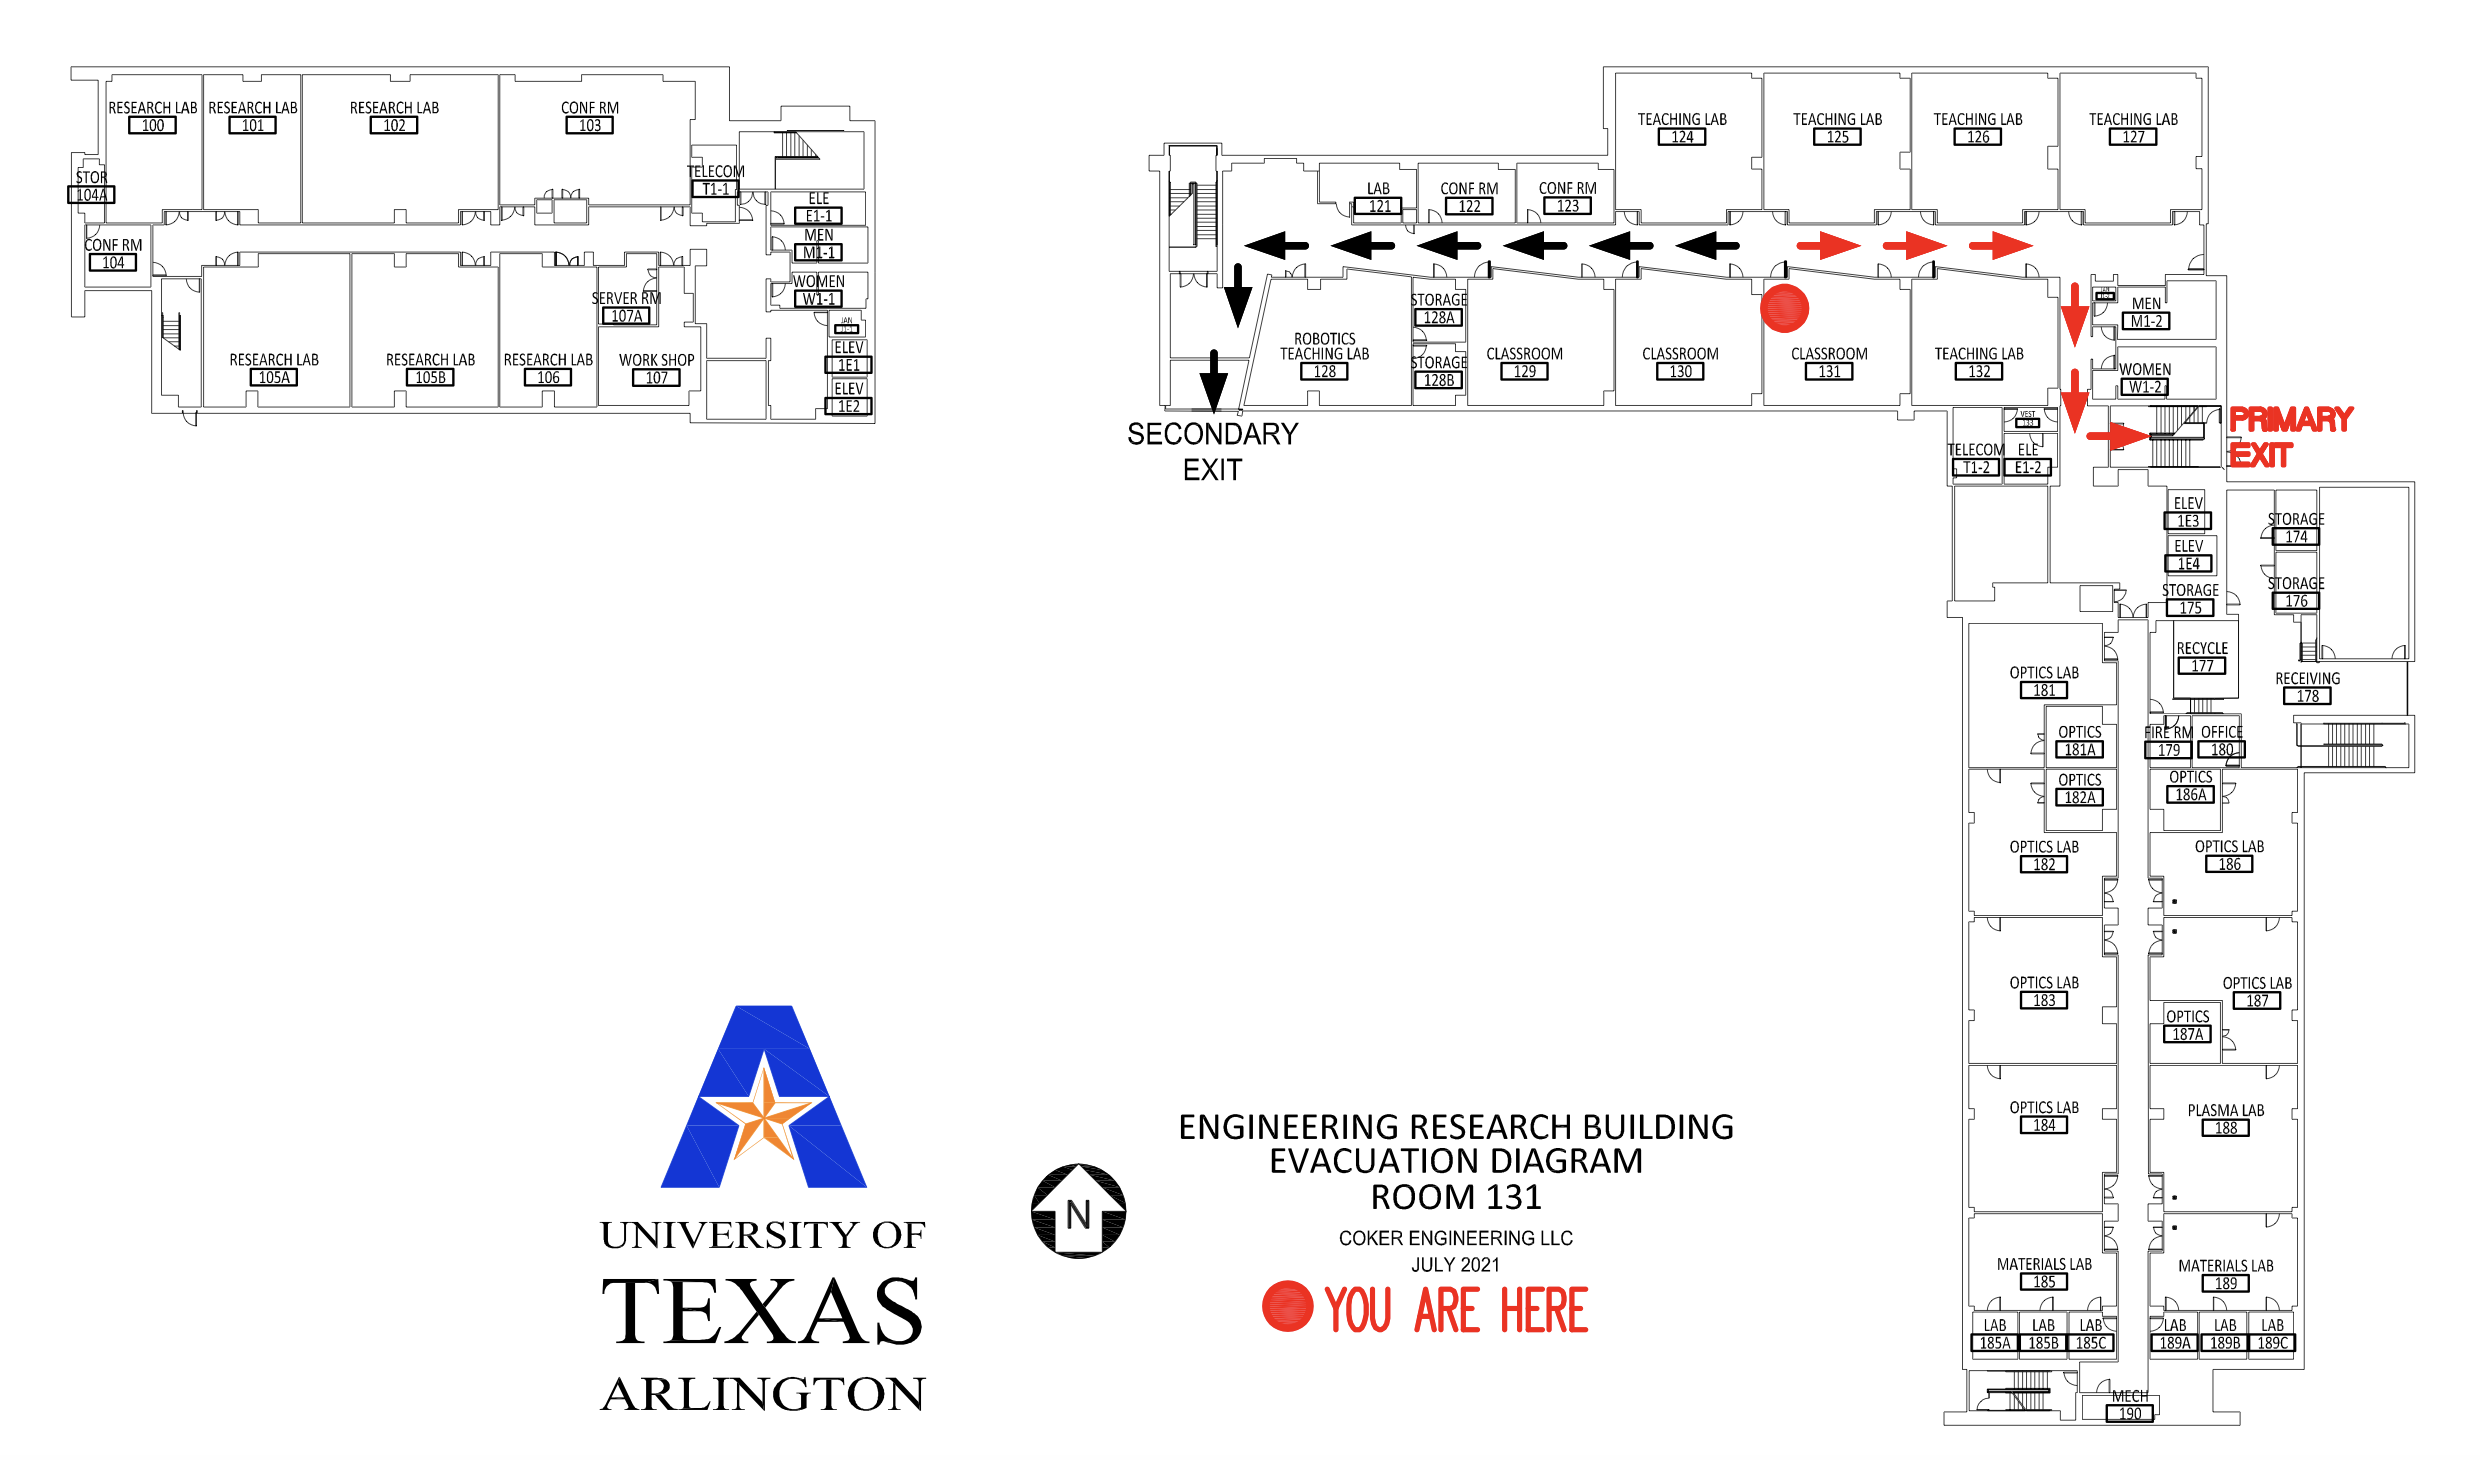
\includegraphics[scale=.4]{source/001/evacuation.png} 

\vskip.25in
\noindent\textbf{Emergency Phone Numbers}:  In case of an on-campus emergency, call the UT Arlington Police Department at 817-272-3003 (non-campus phone), 2-3003 (campus phone). You may also dial 911. Non-emergency number 817-272-3381

%\pagebreak 
\vskip.25in
\noindent\textbf{Final Review Week}: A period of five class days prior to the first day of final examinations in the long sessions shall be designated as Final Review Week. The purpose of this week is to allow students sufficient time to prepare for final examinations. During this week, there shall be no scheduled activities such as required field trips or performances; and no instructor shall assign any themes, research problems or exercises of similar scope that have a completion date during or following this week \textit{unless specified in the class syllabus}.   During Final Review Week, an instructor shall not give any examinations constituting 10\% or more of the final grade, except makeup tests and laboratory examinations. In addition, no instructor shall give any portion of the final examination
during Final Review Week. During this week, classes are held as scheduled. In addition, instructors are not required to limit content to topics that have been previously covered; they may introduce new concepts as appropriate.

\vskip.25in
\noindent\textbf{Course Schedule}: A tentative course schedule can be found on Canvas and below. Keep in mind
that the dates will likely change as the semester progresses and the instructor reserves the right to modify course policies, the course calendar and assignment due dates. \\
\center{
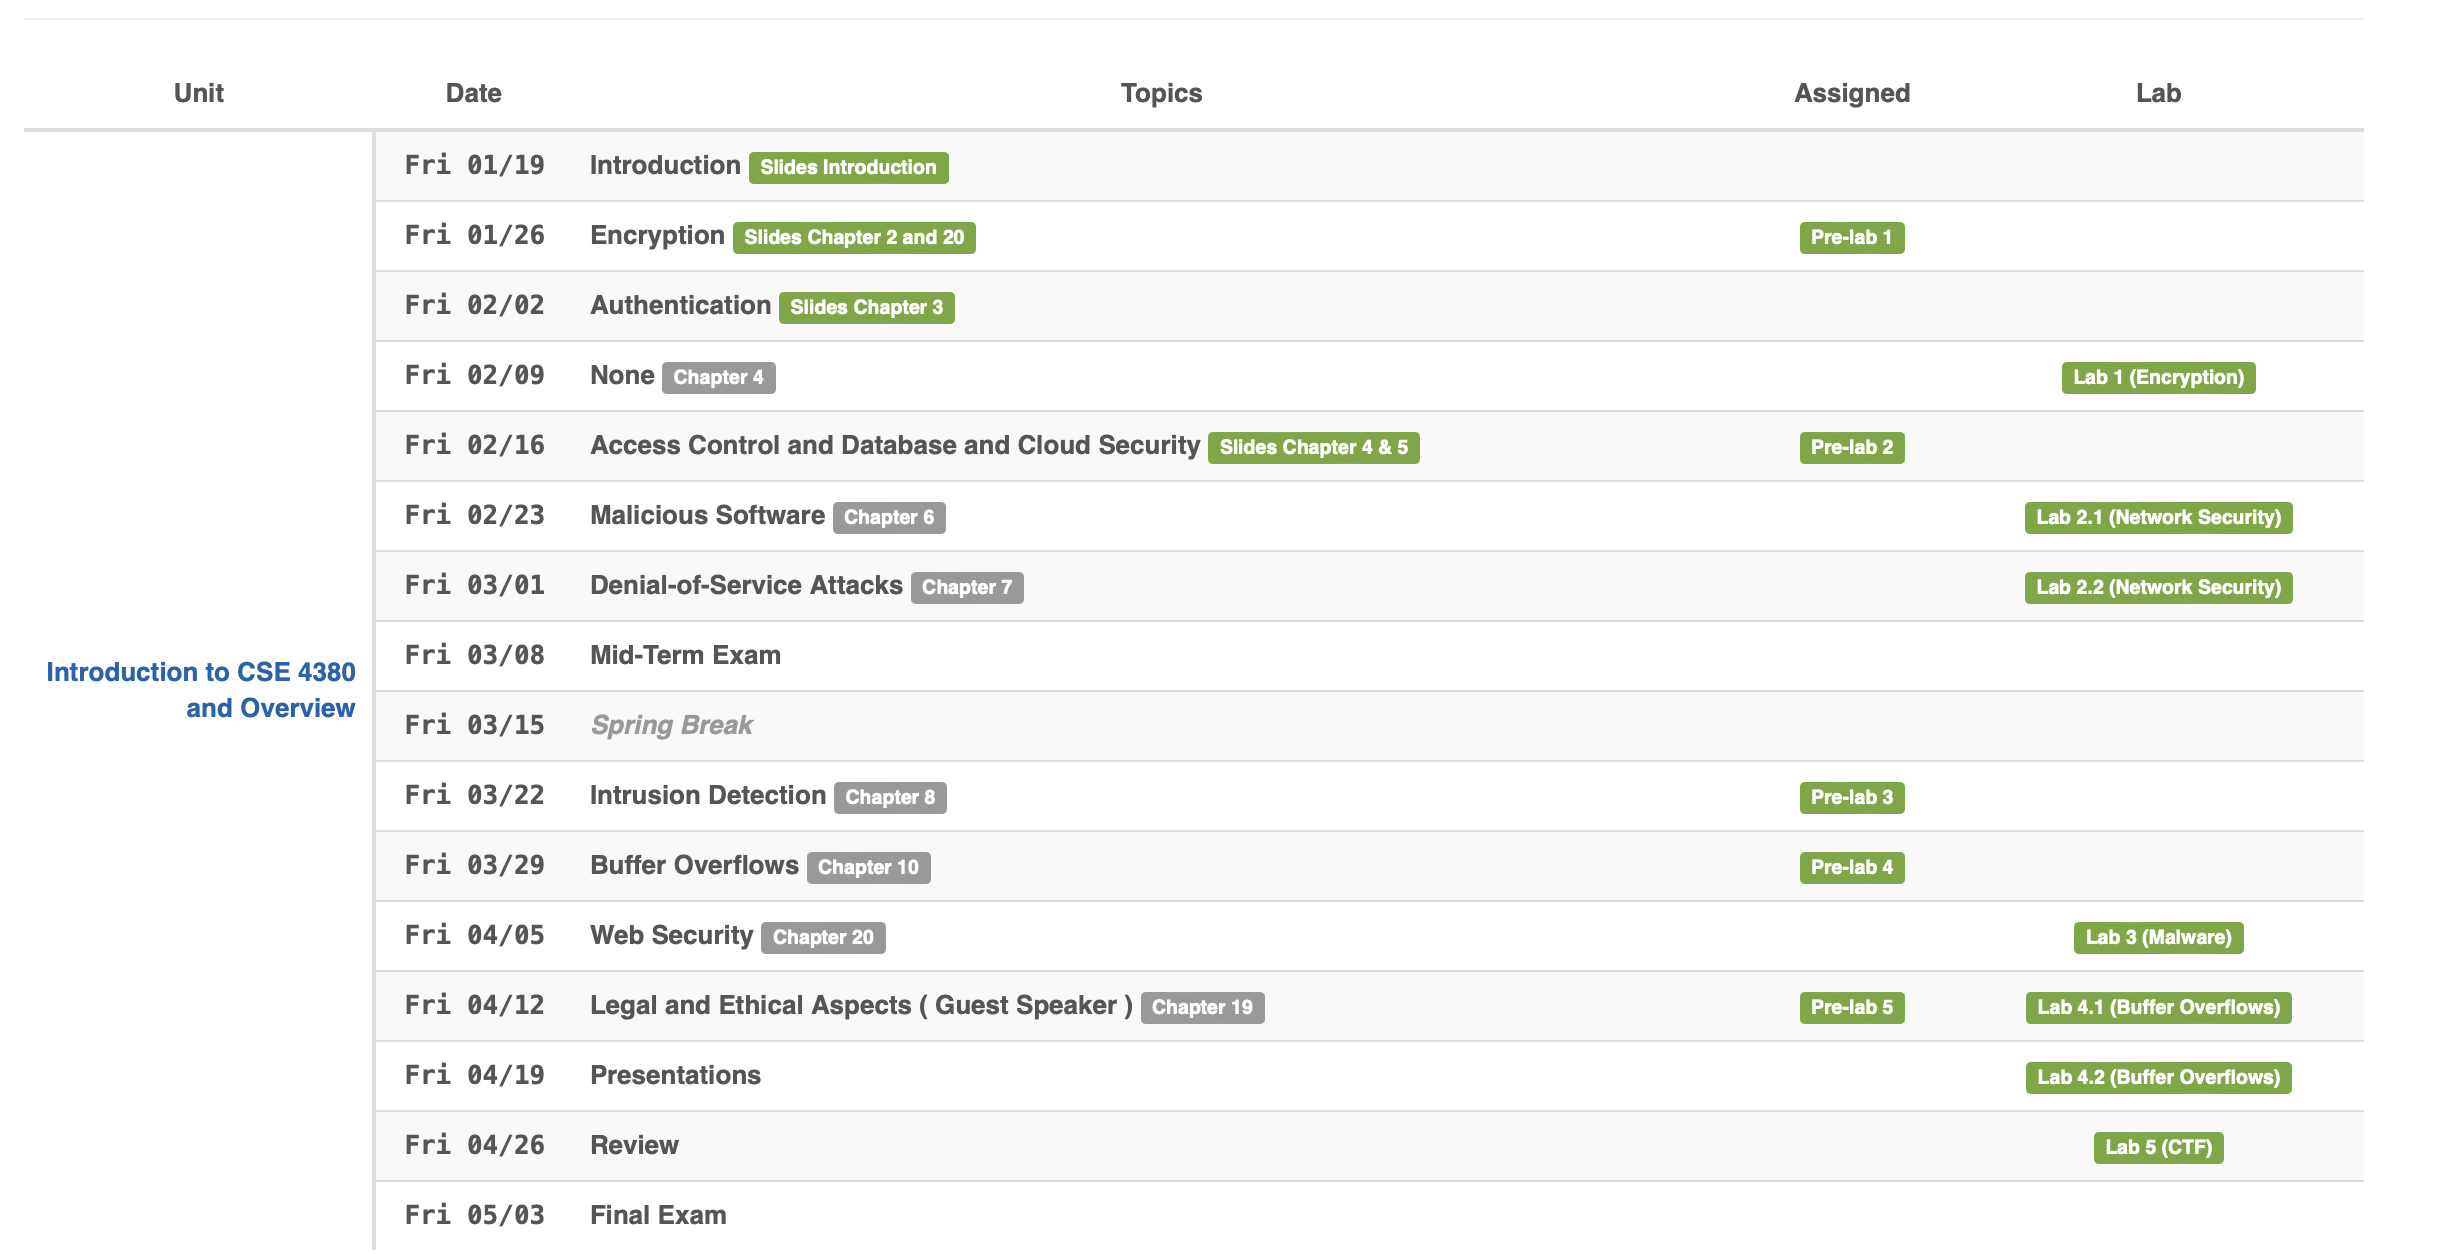
\includegraphics[scale=0.75]{source/001/schedule.png} 
}
\end{document}
